\documentclass{beamer}
\usetheme{}
\usecolortheme{dolphin}           
\useinnertheme{circles}
\setbeamertemplate{itemize items}[default]
\setbeamertemplate{enumerate items}[default]
\usepackage[T1]{fontenc}
\usepackage[utf8]{inputenc}
\usepackage{lmodern}
\usepackage{amsmath}
\usepackage{booktabs} 
\usepackage{graphicx}        
\usepackage{array}
\usepackage{color}
\makeatletter
\def\zapcolorreset{\let\reset@color\relax\ignorespaces}
\def\colorrows#1{\noalign{\aftergroup\zapcolorreset#1}\ignorespaces}
\makeatother
\graphicspath{{/home/swl/Dropbox/ucd/advanced_macro/figures/}} 
\setbeamertemplate{navigation symbols}{}
\setbeamertemplate{footline}[frame number]

%--------------------------------------
\title{Vector Autoregression}
\author{School of Economics, University College Dublin}
\date{Spring 2018}
\begin{document}

%--------------------------------------
\begin{frame}
 \titlepage
\end{frame}
%--------------------------------------

%--------------------------------------
\begin{frame}
  \textbf{Matrix notation}\\
  Consider VAR model with 2 variables, 1 lag  
\begin{align}
  y_{1t} &= a_{11} y_{1, t-1} + a_{12} y_{2,t-1} + \epsilon_{1t}\\ \nonumber
  y_{2t} &= a_{21} y_{1, t-1} + a_{22} y_{2,t-1} + \epsilon_{2t}
\end{align} 
\medskip
 Can write in matrix notation as 
\begin{align}
   \begin{pmatrix}   y_{1t}\\  y_{2t}   \end{pmatrix} &=
   \begin{pmatrix}   a_{11} & a_{12}\\   a_{21} &a_{22}   \end{pmatrix}  \begin{pmatrix}   y_{1,t-1}\\  y_{2,t-1}  \end{pmatrix} +
   \begin{pmatrix}     e_{1t} \\ e_{2t}   \end{pmatrix}   
\end{align}
\begin{align}  Y_t = AY_{t-1} + e_{t} \end{align}
\end{frame}
%--------------------------------------

%--------------------------------------
\begin{frame}
 \textbf{Cumulation of shocks:} VAR expresses variables as function of shocks
 \begin{enumerate}
   \item Yesterday $t-1$
   \item Today $t-1$
 \end{enumerate}
 \medskip
 Shock at $t-1$ depends on shock at $t-1$ and $t-2$, etc.
 \begin{itemize}
   \item Value at $t$ is cumulation of the effect of all shocks from the past
 \end{itemize}
 \medskip
 The fact that the value at $t$ depends on what happened at $t-n$ is useful for generating predictions for $t+1$
\end{frame}
%--------------------------------------

%--------------------------------------
\begin{frame}
  VAR can therefore be represented as \textbf{Vector Moving Average} (VMA):
  \begin{align}
    Y_t &= e_t + AY_{t-1}\\ \nonumber
        &= e_t + A(e_{t-1} + AY_{t-2})\\ \nonumber
        &= e_t + Ae_{t-1} + A^2(e_{t-2} + AY_{t-3})\\ \nonumber
        &= e_t + Ae_{t-1} + A^2e_{t-2} + A^3e_{t-3} + ..... + A^te_0  
  \end{align}
\end{frame}
%--------------------------------------

%--------------------------------------
\begin{frame}
\textbf{Shocks:} Introduce an initial shock and let the error terms be 0 afterwards
\begin{align}  
  e_0&=\begin{pmatrix}   1 \\ 0   \end{pmatrix} \\ 
  e_t&=0\;,t>0 
\end{align}
\medskip
Using VMA representation we get 
\begin{align} 
Y_t = e_t + Ae_{t-1} + A^2e_{t-2} + A^3e_{t-3} + ..... + A^te_0 
\end{align}
\medskip
 Response after $n$ periods will be 
\begin{align}
  A^n \begin{pmatrix} 1 \\ 0  \end{pmatrix}
\end{align}
\medskip
VAR's IRF is directly analogous to AR(1) IRF.
\end{frame}
%--------------------------------------

%--------------------------------------
\begin{frame}
 \textbf{Forecasting:} Given information on $Y_t$ we want to forecast $Y_{t+1}$;
 can model $Y_{t+1}$ as
 \begin{align}  
  Y_{t+1} = AY_t + e_{t+1} 
  \end{align}
  Given $E_te_{t+1}= 0$, an unbiased forecast at time $t$ is $AY_t$ 
  \begin{align} 
  E_tY_{t+1} = AY_t 
  \end{align}
  \begin{itemize}
    \item Similarly, $A^2Y_t$ is an unbiased forecast of $Y_{t+2}$ and $A^nY_t$ of $Y_{t+n}$
  \end{itemize}
  \medskip
  Once estimated, VAR easily used for forecasts  
\end{frame}
%--------------------------------------

%--------------------------------------
\begin{frame}
  \textbf{Semantics:}
  \medskip
  \begin{enumerate}
    \item \textbf{Forecast:} probabilistic statement, usually over a longer time period\\    
    \item \textbf{Prediction:} definitive and specific statement 
  \end{enumerate}
  \medskip
  From \textit{The Signal and the Noise} (Silver, 2012)
\end{frame}
%--------------------------------------

%--------------------------------------
\begin{frame}
  There are many possible VAR models; one we discussed so far is very simple:  
  \begin{itemize}
  \item It doesn't have a constant
  \item Only contains one lagged value
  \end{itemize}
  \medskip
  \textbf{NB-} Can add third variable as constant taking value 1: the equation for the constant term will just state that it equals its own lagged values; this formulation actually incorporates models with constant terms.
\end{frame}
%--------------------------------------

%--------------------------------------
\begin{frame}
  \textbf{Two-lag system:}\\ Using first-order representation
  \begin{align}
    y_{1t} &= a_{11} y_{1, t-1} + a_{12} y_{1,t-2} + a_{13} y_{2, t-1} + a_{14} y_{2,t-2} + \epsilon_{1t}\\
    y_{2t} &= a_{21} y_{1, t-1} + a_{22} y_{1,t-2} + a_{23} y_{2, t-1} + a_{24} y_{2,t-2} + \epsilon_{2t}
  \end{align}
  \medskip
  In matrix form
  \begin{align}  
    Z_t = AZ_{t-1} + e_t 
  \end{align}
  \medskip
  Notation is similar to simpler model, estimation will just be more complex  
\end{frame}
%--------------------------------------

%--------------------------------------
\begin{frame}
  \textbf{Reduced-form:}
  \begin{align*}
    Z_t = AZ_{t-1} + e_t 
  \end{align*}
  \begin{align}
      Z_t= \begin{pmatrix}
      y_{1t} \\ y_{1,t-1} \\ y_{2t} \\ y_{2,t-1}    
      \end{pmatrix};
      A & = \begin{pmatrix}
        a_{11} & a_{12} & a_{13} & a_{14}\\
        1      & 0      & 0      & 0\\
        a_{21} & a_{22} & a_{23} & a_{24}\\
        0      & 0      & 1      & 0    
      \end{pmatrix};
      e_t &= \begin{pmatrix}
        e_{1t} \\ 0 \\ e_{2t} \\ 0 
      \end{pmatrix}
    \end{align}
    \medskip
    The reduced-form VAR is a purely econometric model with no theoretical element.     
\end{frame}
%--------------------------------------

%--------------------------------------
\begin{frame}
  \textbf{Interpreting the model:} given the reduced-form model one interpretation on shocks is that $e_{1t}$ is a shock that only affects $y_{1t}$ on impact and $e_{2t}$ only affects $y_{2t}$
  \begin{itemize}
    \item But what if the shocks has an effect on both $y_{1t}$ and $y_{2t}$?
    \item e.g. aggregate supply and demand shocks affecting inflation and output
  \end{itemize}
  \medskip
  Need to use the reduced-form model to identify structural shocks.
\end{frame}
%--------------------------------------

%--------------------------------------
\begin{frame}
  \textbf{Structural shocks:} Suppose structural and reduced-form shocks are related
  \begin{align}
      e_{1t}&= c_{11}\epsilon_{1t} + c_{12}\epsilon_{2t}\\ \nonumber
      e_{2t}&= c_{21}\epsilon_{1t} + c_{22}\epsilon_{2t}  
  \end{align}
  \begin{align}  
      e_t= C_{\epsilon t} 
  \end{align}
\end{frame}
%--------------------------------------

%--------------------------------------
\begin{frame}
  Can use two VMA representations
\begin{align}
  Y_t &= e_t + Ae_{t-1} + A^2e_{t-2} + A^3e_{t-3} + ..... + A^te_0\\
      &= C_{\epsilon t} +  AC_{\epsilon t-1} + A^2C_{\epsilon t-2} + A^3C_{\epsilon t-3} + ..... + A^tC_{\epsilon 0}
\end{align}
\medskip
Model can be interpreted as
\begin{enumerate}
  \item Shocks $e_t$, IRFs given by $A^n$
  \item Structural shocks $\epsilon_t$, IRFs are given by $A^nC$
  \begin{itemize}
     \item Can be done for any $C$; just don't know the structural shocks.
   \end{itemize} 
\end{enumerate}
\end{frame}
%--------------------------------------

%--------------------------------------
\begin{frame}
  \textbf{Reduced vs. Structural shocks:}\\
  Consider contemporaneous interactions between variables
\begin{align}
  y_{1t} &= a_{12}y_{2t} + b_{11}y_{1,t-1} + b_{12}y_{2,t-1} +\epsilon_{1t}\\ \nonumber
  y_{2t} &= a_{21}y_{1t} + b_{21}y_{1,t-1} + b_{22}y_{2,t-1} +\epsilon_{1t}
\end{align}
  \begin{align}  
    AY_t = BY_{t-1} + \epsilon_t 
  \end{align}
  \begin{align}
   A= \begin{pmatrix}
      1 & -a_{12}\\ -a_{21} & 1 \\
    \end{pmatrix}
  \end{align}
\end{frame}
%--------------------------------------

%--------------------------------------
\begin{frame}
  Reduced-form model
  \begin{align}
    Y_t= DY_{t-1} + e_t
  \end{align}
  \medskip
  Has following coefficients and shocks
\begin{align}
  D &= A^{-1}B \\
  e_t &= A^{-1} \epsilon_t   
\end{align}
\end{frame}
%--------------------------------------

%--------------------------------------
\begin{frame}
  Structural model, impulse response to structural shocks from $n$ periods given by
  \begin{align}
    D^nA^{-1}
  \end{align}
  \medskip
  Hold for any arbitrary $A$ matrix
  \begin{align}
  Y_t&= e_t + De_{t-1} + D^2e_{t-2} + D^3e_{t-3} + .....\\ \nonumber
     &= A^{-1}\epsilon_t + DA^{-1}\epsilon_{t-1} + D^2A^{-1}\epsilon_{t-2} + D^3A^{-1}\epsilon_{t-3} + ..... \end{align}
\end{frame}
%--------------------------------------

%--------------------------------------
\begin{frame}
  \textbf{'What-if'}: for reduced-form VAR the question  
  \begin{quote}
    What happens if there is a shock to the first variable in the VAR?  
  \end{quote}
  \medskip
  Becomes   
  \begin{quote}
    What will normally happen if there is a shock to the first variable, given that this is usually associated with a corresponding shock to the second variable?    
  \end{quote}
  \medskip
  Due to correlation of error series in reduced-form VAR: often interested in different shock types that are uncorrelated
  \begin{itemize}
    \item Structural identification how reduced-form shocks are actually combinations of uncorrelated structural shocks
  \end{itemize}
\end{frame}
%--------------------------------------

%--------------------------------------
\begin{frame}
  \textbf{Structural VAR}
  \begin{align}  
  AY_t = BY_{t-1} + C\epsilon_t 
  \end{align}
  \medskip
  Number of parameters in the model is
  \begin{align}
    3n^2 + \frac{n(n+1)}{2}
  \end{align}
  \begin{enumerate}
    \item $n^2$ parameters in $A$
    \item $n^2$ parameters in $B$
    \item $n^2$ parameters in $C$
    \medskip
    \item $\frac{n(n+1)}{2}$ parameters in $\sum$
  \end{enumerate}
\end{frame}
%--------------------------------------

%--------------------------------------
\begin{frame}
  \textbf{Estimation}\\  
  \begin{align}  
  Y_t = DY_{t-1} + e_t 
  \end{align}
  \medskip
  Provides information on $n^2+\frac{n(n+1)}{2}$ parameters
  \begin{enumerate}
    \item Parameters in $D$
    \item Estimated covariance matrix for the reduced-form errors
  \end{enumerate}
  \medskip
  Need to impose $2n^2$ \textit{a priori} theoretical restrictions on the structural VAR.  
\end{frame}
%--------------------------------------

%--------------------------------------
\begin{frame}
  Imposing $2n^2$ restrictions will leave 
  \begin{align}
    n^2+\frac{n(n+1)}{2}
  \end{align}
  \medskip
  known reduced-form parameters and equal number of structural parameters that we like to know; can get an unique solution here.
  \begin{itemize}
    \item $n^2+\frac{n(n+1)}{2}$ equations in $n^2+\frac{n(n+1)}{2}$ unknowns
  \end{itemize}
  \medskip
  e.g. can assume that reduced-form VAR is equal to SVAR
  \begin{align}
    A=C=I
  \end{align}
\end{frame}
%--------------------------------------

%--------------------------------------
\begin{frame}
  \textbf{Recursive SVAR:} SVARs identify shocks as coming from distinct independent sources (uncorrelated).
  \begin{itemize}
    \item How to get uncorrelated structural shocks from correlated reduced form shocks?
  \end{itemize}
  \medskip
  Reduced-form errors are combinations of set of independent structural errors
  \begin{align*}
    Y_t &= DY_{t-1} + e_t\\ 
    e_t &= A^{-1} \epsilon_t \\\\ 
    AY_t &= BY_{t-1} + C\epsilon_t  
  \end{align*}
  \begin{enumerate}
    \item Set $A = I$
    \item Construct $C$ such that structural shocks will be uncorrelated
  \end{enumerate}
\end{frame}
%--------------------------------------

%--------------------------------------
\begin{frame}
  \textbf{Identification:} Take reduced-form VAR with error series ($e_{1t}$ , $e_{2t}$, $e_{3t}$); Assume that one variable is first structural shock
  \begin{align}
    \epsilon_{1t} = e_{1t} 
  \end{align}
  \medskip
  Run following two regression involving reduced-form shocks
  \begin{align}
    e_{2t} &= c_{21}e_{1t} + \epsilon_{2t}\\
    e_{3t} &= c_{31}e_{1t} + c_{32}e_{2t} + \epsilon_{3t}  
  \end{align}  
\end{frame}
%--------------------------------------

%--------------------------------------
\begin{frame}
  This produces
  \begin{align}
    Ge_t= \epsilon_t
  \end{align}
  \medskip
  Invert $Ge_t$ to create $C$ and give
  \begin{align}
    e_t= C\epsilon_t
  \end{align}
  \medskip
  Identification: Done
  \begin{itemize}
    \item Recall that in OLS the error terms are uncorrelated with RHS variables: here by construction, we have that $\epsilon_t$ are uncorrelated with each other
  \end{itemize}  
\end{frame}
%--------------------------------------

%--------------------------------------
\begin{frame}
  \textbf{Cholesky decomposition:} Posits causal chain of shocks and creates a lower-triangular matrix
  \medskip
  \begin{enumerate}
  \item First shock affects all variables at time $t$
  \item Second only affects two of them at time $t$
  \item Last shock only affects one variable at time $t$
\end{enumerate} 
\end{frame}
%--------------------------------------

%--------------------------------------
\begin{frame}
 Two important issues with using Cholesky decomposition: \medskip
 \begin{enumerate}
   \item Restriction assumptions: variables are sticky and do not respond immediately to some shocks
   \item Ordering: not unique meaning that there are $n!$ possible recursive orderings
 \end{enumerate} 
\end{frame}
%--------------------------------------

%--------------------------------------
\begin{frame}
  \textbf{Ordering:} Some variables only having effect on some variables at time $t$
  \begin{itemize}
    \item Let $C=I$, estimate $A$ and $B$ using OLS.
  \end{itemize}
   
\begin{align}
  y_{1t} &= b_{11}y_{1,t-1} + b_{12}y_{2,t-1} + b_{13}y_{3,t-1} + \epsilon_{1t}\\ \nonumber
  y_{2t} &= b_{21}y_{1,t-1} + b_{22}y_{2,t-1} + b_{23}y_{3,t-1}-a_{21}y_{1t} + \epsilon_{2t}\\ \nonumber
  y_{3t} &= b_{31}y_{1,t-1} + b_{32}y_{2,t-1} + b_{33}y_{3,t-1}-a_{31}y_{1t} - a_{32}y_{2t} + \epsilon_{3t}
\end{align}
  \medskip 
  Different combinations of $A$, $B$ and $C$ can deliver the same structural model. 
\end{frame}
%--------------------------------------

%--------------------------------------
\begin{frame}
  \textbf{OLS:} VAR is set of linear equations
  \begin{itemize}
    \item $n$-variable and $n$-equation model where each variable is explained by its lagged value and the current and lagged value of the $n-1$ remaining variables
  \end{itemize}
  \medskip
  OLS would be obvious technique for estimating coefficients; however it will produce biased estimates
\end{frame}
%--------------------------------------

%--------------------------------------
\begin{frame}  
\begin{align}
  y_t= \rho y_{t-1} + \epsilon_t
\end{align}
 For AR(1) model, the OLS estimator for sample size $T$ is
\begin{align}
  \hat{\rho} &= \frac{\sum^T_{t=2}y_t y_{t-1}}{\sum^T_{t=2}y^2_{t-1}}\\ \nonumber
  &= \rho + \frac{\sum^T_{t=2}\epsilon_t y_{t-1}}{\sum^T_{t=2}y^2_{t-1}}=
  \rho + \sum_{t=2}^T \left(\frac{y_{t-1}}{\sum_{t=2}^T y^2_{t-1}} \right) \epsilon_t
\end{align}
\medskip

\end{frame}
%--------------------------------------

%--------------------------------------
\begin{frame}
 \begin{enumerate}
   \item $\epsilon_t$ is independent of $y_{t-1}$ 
   \begin{align}
    \mathop{\mathbb{E}}(y_{t-1}\epsilon_t)= 0  
 \end{align}
   \item $\rho>0$: positive shock to $\epsilon_t$ will increase current and future values of $y_t$.
 \end{enumerate}
 \medskip
 $y_t$ is a function of $\epsilon_t$: $\epsilon_t$ is not independent of $\sum^T_{t=2}y^2_{t-1}$
 \begin{align}
     \mathop{\mathbb{E}} \hat{\rho}<\rho
   \end{align} 
 Due to negative correlation between $\epsilon_t$ and $\frac{y_{t-1}}{\sum_{t=2}^T y^2_{t-1}}$ 
\end{frame}
%--------------------------------------

%--------------------------------------
\begin{frame}
 \textbf{Size of bias} depends on two factors \medskip
 \begin{enumerate}
  \item The size of $\rho$: The bigger this is, the stronger the correlation of the shock with future values and thus the bigger the bias.
  \item Sample size $T$: The larger this is, the smaller the fraction of the observations sample that will be highly correlated with the shock and thus the smaller the bias.
\end{enumerate}
\end{frame}
%--------------------------------------

%--------------------------------------
\begin{frame}
  \textbf{Bootstrapping:} 
   Use OLS to estimate model 
   \begin{align}
     Z_t= AZ_{t-1} + \epsilon_t
   \end{align}
   \medskip
   Save errors $\hat{\epsilon_t}$ and randomly sample error series $\epsilon^*_t$ and simulated data
   \begin{align}
     Z^*_t= \hat{A}Z^*_{t-1} + \epsilon^*_t
   \end{align}
   \medskip
    Estimate VAR with simulated data; save coefficients $\hat{A}^*$
    \begin{itemize}
      \item Compute median for each $\hat{A}^*$: $\bar{A}$; compare to $\hat{A}$ to get estimate of OLS bias
    \end{itemize}
    \medskip
    Can construct new estimates 
    \begin{align}
      A^{boot} = \hat{A}-(\bar{A}-\hat{A})
    \end{align}  
\end{frame}
%--------------------------------------


%--------------------------------------
\begin{frame}
  \textbf{Maximum Likelihood Estimation}: estimator that maximises the value of the likelihood function for the observed data, for parameter set $\theta$
  \begin{align}
    f(y_1,y_2,.....,Y_n| \theta)
  \end{align}
  \medskip
  Similar to OLS, MLE estimates are biased but they are also
  \begin{enumerate}
    \item Consistent
    \item Asymptotically efficient
  \end{enumerate}  
\end{frame}
%--------------------------------------

%--------------------------------------
\begin{frame}  
  \textbf{Joint likelihood:} ML estimates are given by multiplying likelihood of each observation; maximising joint likelihood  
\begin{align}
  f(y_1,...,y_n| \mu, \sigma) &= \prod^n_{i=1} \frac{1}{\sqrt{2\pi \sigma^2}} exp \left [ \frac{-(y_i-\mu)^2)}{2\sigma^2} \right ] \\ \nonumber
  &= \prod^n_{i=1} f(y_i| \theta)\\
  log \;f(y_1,...,y_n| \mu, \sigma) &= -\frac{n}{2} log 2\pi - n log \sigma + \sum^n_{i=1} \left [ \frac{-(y_i-\mu)^2}{2\sigma^2} \right ] \\ \nonumber
  &= \sum^n_{i=1} ln\; f(y_i| \theta)
\end{align}\
\end{frame}
%--------------------------------------

%--------------------------------------
\begin{frame}
  Consider AR(1) model
  \begin{align}
  y_t&= \rho y_{t-1} + \epsilon_t \\ 
   \epsilon_t &\sim N(0, \sigma^2)
  \end{align}
  For joint unconditional series $y_1,y_2,...,y_n$ we assume
  \begin{align}
     y_2\sim N(\rho y_1,\sigma^2), y_3\sim N(\rho y_2,\sigma^2),... 
   \end{align} 
   \medskip  
  For $\theta= (\rho, \sigma)$, conditional on the first observation the joint distribution can be written as
\begin{align}
  f(y_2,...,y_n| \theta, y1) &= \prod^n_{i=2} \frac{1}{\sqrt{2 \pi \sigma^2}} exp \left [ \frac{-(y_i - \rho y_{i-1})^2}{2\sigma^2} \right ] \\
  log f(y_2,...,y_n| \theta, y1) &= -\frac{n}{2} log 2\pi - n log \sigma + \sum^n_{i=1} 
  \left [ \frac{-(y_i-\rho y_{i-1})^2}{2\sigma^2} \right ]\\ \nonumber
  &=  -\frac{n}{2} log 2\pi - n log \sigma - \frac{1}{2\sigma^2} \sum^n_{i=1}(y_i-\rho y_{i-1})^2
\end{align}
\end{frame}
%--------------------------------------

%--------------------------------------
\begin{frame}
 \textbf{Parameters:} For VAR with $n$ variables and $k$ lags, number of parameters equals
 \begin{align}
   n^2k + \frac{n(n-1)}{2} 
 \end{align}
 \begin{itemize}
   \item $n=3,k=1$: 12 parameters
   \item $n=6,k=6$: 231 parameters
 \end{itemize}
 \medskip
 Two issues to consider
 \begin{enumerate}
   \item Many coefficients are probably zero (or close)
   \begin{itemize}
     \item Overfitting: poor-quality estimates, bad forecasts
   \end{itemize}
   \item Can limit the number of variables/lags used
   \begin{itemize}
      \item Misspecification: poor inferences, bad forecasts
    \end{itemize} 
 \end{enumerate}
\end{frame}
%--------------------------------------

%--------------------------------------
\begin{frame}
  \textbf{Bayesian modeling:} Can incorporate additional information about coefficients to produce models that are not as highly sensitive to the features of the particular data sets we are using   
  \begin{align}
    P(A|B) &= \frac{P(B|A)P(A)}{P(B)}\\
    P(A|B)&\propto P(B|A)P(A)
  \end{align}
  \medskip
  Can use \textbf{Bayes' Law} to incorporate prior knowledge.
\end{frame}
%--------------------------------------

%--------------------------------------
\begin{frame}
 For the set of variables $Z$ and parameters $\theta$
\begin{align}
  P(\theta= \theta^* | Z=D) \propto P(Z=D | \theta =\theta^*)P(\theta= \theta^*)  
\end{align}
\medskip
In English: the probability data parameters $\theta$ take on value $\theta^*$ given data $D$ is a function of
\begin{enumerate}
  \item The probability that $Z=D$ if $\theta= \theta^*$
  \item The probability that $\theta = \theta^*$
\end{enumerate}
\end{frame}
%--------------------------------------

%--------------------------------------
\begin{frame}
  \textbf{Probability density function:} Rewrite relationship given that data and coefficients are continuous  
  \begin{align}
    f_\theta(\theta^* | D) \propto f_Z(D | \theta^*)f_\theta(\theta^*)
\end{align}
 Model has three important components
 \begin{enumerate}
   \item Likelihood function
   \item Parameters
   \item Prior
 \end{enumerate}  
\end{frame}
%--------------------------------------

%--------------------------------------
\begin{frame}
  \textbf{Likelihood function:} 
  \begin{align}
    f_Z(D | \theta^*)
  \end{align}
    For each possible value of $\theta^*$ gives the probability of observed dataset if true coefficients
    \begin{align}
      \theta= \theta^*
    \end{align}    
    The likelihood function can be calculated once you have made assumptions about the distributional form of the error process.    
\end{frame}
%--------------------------------------

%--------------------------------------
\begin{frame}
  \textbf{Prior:} Summarises the researcher's pre-existing knowledge about the parameters $\theta$, specified as distribution 
  \begin{align}
    f_\theta(\theta^*)
  \end{align}
  Prior distribution is combined with the likelihood function to produce posterior distribution
    \begin{align}
      f_\theta(\theta^* | D)
    \end{align}
    Specifies the probability of all possible coefficient values given both the observed data and the priors    
\end{frame}
%--------------------------------------


%--------------------------------------
\begin{frame}
  \textbf{Point estimate:} For best estimator can use mean of posterior distribution 
\begin{align}
  \hat{\theta}= \int^\infty_{-\infty} xf_\theta(x | D)dx
\end{align}
 Estimator is weighted average of
 \begin{enumerate}
   \item The maximum likelihood estimator
  \item The mean of the prior distribution
 \end{enumerate}
 With normally distributed errors Bayesian estimators of VAR coefficients are weighted averages of OLS coefficients and the mean of the prior distribution 
\end{frame}
%--------------------------------------

%--------------------------------------
\begin{frame}
  \textbf{Long-run restrictions:} Identifying assumptions for VAR requires knowledge on how variables react instantaneous to certain shocks
  \begin{itemize}
    \item Variables can be slow or information available with lag
    \item Economic theory of little help due to focus on long run
    \begin{itemize}
      \item Positive aggregate demand shock will on the long-run have no effect on output and positive effect on price level
    \end{itemize}
  \end{itemize}
  \medskip
  Alternative approach: use theoretically-inspired long-run restrictions to identify shocks and impulse responses.
\end{frame}
%--------------------------------------

%--------------------------------------
\begin{frame}
  \begin{align}
    Z_t&= BZ_{t-1}+C\epsilon_t    
  \end{align}
  Covariance matrix of structural shocks is
  \begin{align}
    E(\epsilon_t \epsilon_t') &= \begin{pmatrix} E(\epsilon_1^2) & E(\epsilon_1 \epsilon_2) \\ E(\epsilon_1 \epsilon_2) & E(\epsilon_2^2) \end{pmatrix} = I
  \end{align}
  \medskip
  Structural shocks are uncorrelated and have unit variance.\\
  Reduced-form:
  \begin{align}
    \sum = E(e_t e_t') = E \{(C\epsilon_t) (C\epsilon_t)'\} = CE(\epsilon_t \epsilon_t')C' = CC'
  \end{align}
  Observed covariance structure of the reduced-form shocks provide information on how they are related to uncorrelated structural shocks
\end{frame}
%--------------------------------------

%--------------------------------------
\begin{frame}
  \textbf{Long-run effects SVAR}
  \begin{align}
    Z_t=(\Delta y_t,\Delta x_t)'
  \end{align}
  Long-run effect of shock on $y_t$ is sum of effects on 
  \begin{align}
    \Delta y_t, \Delta y_{t+1},\Delta y_{t+1},...,\Delta y_{t+n}
  \end{align}
  i.e. long-run effect is sum of impulse responses, meaning that for model     
  \begin{align}
    Z_t = BZ_{t-1} + C\epsilon_t
  \end{align}
  The impulse response is
  \begin{enumerate}
    \item $C$ in $t$
    \item $BC$ in $t+1$
    \item $B^nC$ after $n$ periods
  \end{enumerate}  
\end{frame}
%--------------------------------------

%--------------------------------------
\begin{frame}
  \textbf{Long-run level effect}  
  \begin{align}
    D=(I+B+B^2+B^3+...)C
  \end{align}
  With $B$'s eigenvalues within unit circle 
  \begin{align}
    I+B+B^2+B^3+...=(I-B)^{-1}
  \end{align}
  This becomes
  \begin{align}
  D=(I-B)^{-1}C
  \end{align}
\end{frame}
%--------------------------------------

%--------------------------------------
\begin{frame}
  \textbf{Blanchard-Quah method:}
  \begin{align}
    DD'=(I-B)^{-1}CC'\left( (I-B)^{-1} \right)'
  \end{align}
  We defined the covariance matrix of reduced-form shocks as
  \begin{align}
    CC'= \sum 
  \end{align}
  \medskip
  This can be estimated, producing
  \begin{align}
    DD'=(I-B)^{-1}\sum \left( (I-B)^{-1} \right)'
  \end{align} 
\end{frame}
%--------------------------------------

%--------------------------------------
\begin{frame}
\textbf{Long-run effect restriction:} Assume that $D$ is lower-triangular
\medskip  
  \begin{enumerate}
    \item First shock has long-run effect on first variable
    \item First and second shock have long run effect on second variable
    \item etc.
  \end{enumerate}
  \begin{align}
    D= \begin{pmatrix} d_{11} & 0 \\ d_{21} & d_{22} \end{pmatrix}
  \end{align}
\end{frame}
%--------------------------------------

%--------------------------------------
\begin{frame}
  \textbf{Cholesky factor:} All symmetric matrices have a unique lower-diagonal matrix $D$ such that $DD'$ equals the symmetric matrix
  \begin{itemize}
    \item Symmetrix matrix means that entry $i,j$ equals entry $j,i$
  \end{itemize}
  \medskip
  Calculate $D$ using known matrix
  \begin{align}
    (I-B)^{-1}\sum \left( (I-B)^{-1} \right)'
  \end{align}
  Given 
  \begin{align}
    D=(I-B)^{-1}C
  \end{align}
  Matrix $C$ defining structural shocks can be calculated as  
  \begin{align}
    C=(I-B)D
  \end{align}
\end{frame}
%--------------------------------------

%--------------------------------------
\begin{frame}
  \textbf{Galí} (1999): Looks at change in labour productivity versus number of hours worked
  \begin{itemize}
    \item Based on Real Business Cycle (RBC) model which assumes that technology shocks drive business cycle
    \item In this case hours worked should increase in booms compared to recessions
  \end{itemize}
  \medskip
  Lower-diagonal assumption is that technology shock can affect productivity in long-run, but non-technology shock cannot
\end{frame}
%--------------------------------------

%--------------------------------------
\begin{frame}
  \begin{figure}
    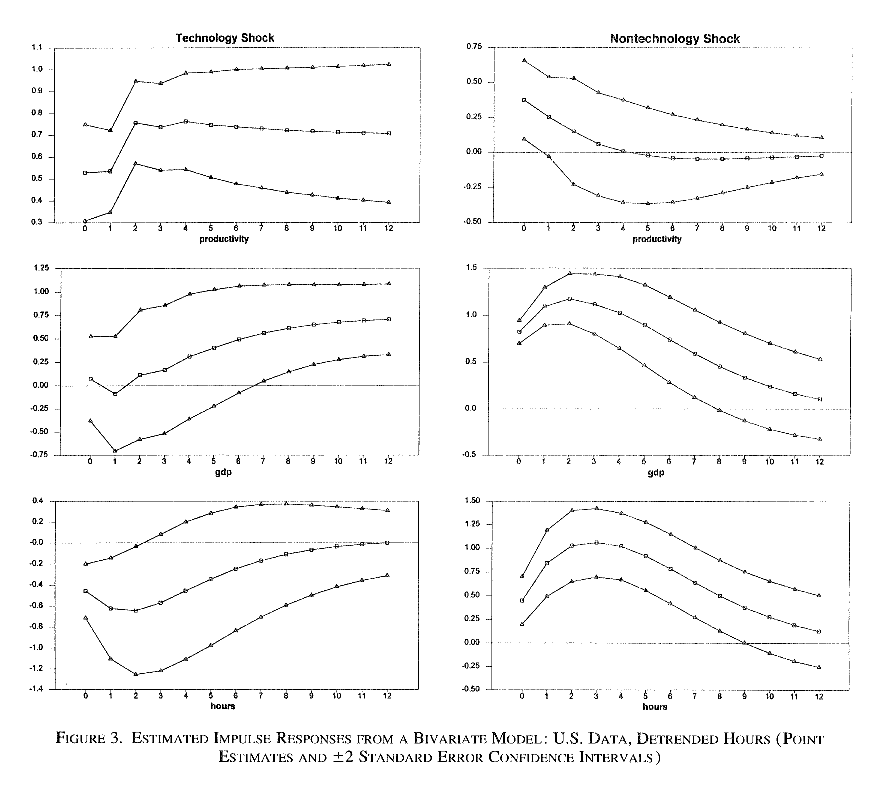
\includegraphics[scale=.7]{gali.eps}
  \end{figure}
\end{frame}
%--------------------------------------

%--------------------------------------
\end{document}
